\documentclass[12pt]{article}
\usepackage{amsmath,amssymb,enumerate,enumitem}%la base
\usepackage{fancyhdr}%pour custom les en-têtes et pieds de page
\usepackage[table]{xcolor}%pour les couleurs
\usepackage[a4paper,lmargin=1cm,rmargin=1cm,tmargin=1cm,bmargin=2cm]{geometry}
\usepackage[T1]{fontenc}
\usepackage{hyperref}%hyperliens
\usepackage{graphicx}%images
\usepackage[most]{tcolorbox}%pour les encadrés
\usepackage{import} % pour importer
\usepackage{listings}%pour afficher du code R
\usepackage[pages=some]{background} % pour la page de garde
\usepackage{subcaption}

% --- Couleur violet thème ---
\definecolor{ensae}{RGB}{71, 1, 125}

\hypersetup{
    colorlinks = true,
    linkcolor = ensae!70!white,
    filecolor = ensae,      
    urlcolor = ensae,
    pdfpagemode = FullScreen,
    pdftitle = Linear Time Series Assignment,
    pdfauthor = Alban Géron
}

\pagestyle{fancy}
\lhead{} \rhead{} \lfoot{} \rfoot{}
\renewcommand{\headrulewidth}{0pt}\renewcommand{\footrulewidth}{0pt}

% --- Configuration R ---
\definecolor{codegreen}{rgb}{0,0.6,0}
\definecolor{codegray}{rgb}{0.5,0.5,0.5}
\definecolor{customyellow}{rgb}{1,1,0}
\lstset{
    language=R,                         % R par défaut
    commentstyle=\color{codegreen},
    keywordstyle=\color{blue},
    numberstyle=\tiny\color{codegray},
    stringstyle=\color{magenta},
    basicstyle=\ttfamily,
    breakatwhitespace=false,         
    breaklines=true,                 
    captionpos=b,                    
    keepspaces=true,                 
    numbers=left,                    
    numbersep=3pt,                  
    showspaces=false,                
    showstringspaces=false,
    showtabs=false,                  
    tabsize=2,
    literate=%
        {é}{{\'e}}1 {è}{{\`e}}1 {à}{{\`a}}1 {ù}{{\`u}}1 {â}{{\^a}}1 {ê}{{\^e}}1 {î}{{\^i}}1 {ô}{{\^o}}1 {û}{{\^u}}1
        {É}{{\'E}}1 {È}{{\`E}}1 {À}{{\`A}}1 {Ù}{{\`U}}1 {Â}{{\^A}}1 {Ê}{{\^E}}1 {Î}{{\^I}}1 {Ô}{{\^O}}1 {Û}{{\^U}}1
        {ç}{{\c{c}}}1 {Ç}{{\c{C}}}1
}
\newcommand\rcode[1]{{\lstinline[language=R]!#1!}}

% --- Titres ---
\usepackage{titlesec}
\renewcommand{\thesection}{\Roman{section}} % Titres sections en chiffres romains
\titleformat{\section}{\normalfont\sffamily\bfseries\Large}{\thesection}{1em}{}
\titleformat{\subsection}{\normalfont\sffamily\bfseries\large}{\thesubsection}{1em}{}
\titleformat{\subsubsection}{\normalfont\sffamily\bfseries}{\thesubsubsection}{1em}{}
\setlist[enumerate]{
    font = \color{ensae!70!white}\sffamily,
    leftmargin = *,
    resume
}

% --- Macros ---
\newcommand{\ARMA}{\textsf{ARMA}}
\newcommand{\ARIMA}{\textsf{ARIMA}}
\newcommand{\AIC}{\textsf{AIC}}
\newcommand{\BIC}{\textsf{BIC}}
\newcommand{\WN}{\textsf{WN}}



\begin{document}
    \backgroundsetup{
        scale = 1,
        angle = 0,
        opacity = 1,
        contents = {
            
\includegraphics[width = \paperwidth, height = \paperheight, keepaspectratio]{bgcover.pdf}
        }
    }
   \BgThispage
    \newgeometry{
        lmargin=1cm,
        rmargin=7cm,
        tmargin=4cm,
        bmargin=4cm
    }
    \thispagestyle{empty} % pas de numérotation pour cette page
    \begin{center}
        
\includegraphics[width=0.8\textwidth]{ensae IP paris.png}

        \vskip4cm

        \Large\bfseries
        \begin{tcolorbox}[
            enhanced, sharp corners,
            colback = ensae!5!white,
            colframe = ensae!60!white,
            boxrule = 0.5pt,
            drop fuzzy shadow = gray
        ]
            \centering {\huge\sffamily ARIMA modelling of a time series}

            \vskip0.3cm

            \emph{\Large Linear Time Series Assignment}
        \end{tcolorbox}

        \vskip4cm

        Alban \textsc{Géron} and Théo \textsc{Lartigau}

        \vskip0.5cm

        Academic year: 2024-2025
    \end{center}

    \newpage
    \restoregeometry

    \section{The data}

    \begin{enumerate}
        \item The chosen series is the \emph{seasonally and working-day adjusted Industrial Production Index (IPI) for the manufacture of beverages}\footnote{\url{https://www.insee.fr/fr/statistiques/serie/010767669}}. It tracks the monthly physical output of France’s drinks industry (breweries, wineries, distillers, soft‑drink plants and bottled‑water facilities), adjusted for calendar and seasonal fluctuations. The index is expressed on a base‑$100$ scale with 2021 as the reference year, that is, a value of $110$ means the beverage industry produced $10 \%$ more than its 2021 average in that month.

        To isolate the monthly industrial production data, rows should be filtered to retain only those whose first column matches the \texttt{YYYY-MM} format. The second column, containing the index values, should then be extracted and converted to numeric form. Because the data appears in reverse chronological order, the values should be reversed to restore proper temporal sequencing.

        Although the base‑$100$ scaling tends to keep the variance relatively stable, a logarithmic transformation may still be considered if volatility appears to increase with the level of the index.

        \item As a first step we have checked the stationarity of the initial series, which we will label $(Y_t)$ in the following. Table \ref{tab:stationarity_tests} summarizes the results of the Augmented Dickey-Fuller (ADF), Phillips-Perron (PP) and Kwiatkowski-Phillips-Schmidt-Shin (KPSS) tests. The results of the three stationarity tests on the initial series are somewhat contradictory. Both the ADF and PP tests reject the null hypothesis of a unit root at the $5 \%$ level, suggesting that the series is stationary. However, the KPSS test rejects the null hypothesis of level stationarity, indicating that the series is not stationary. This discrepancy calls into question the stationarity of $(Y_t)$. To determine the integration order of $(Y_t)$, we test the stationarity of the first-order differenced series $(\nabla Y_t)$. Plotting the series $(\nabla Y_t)$ shows that it seems stationary, see Figure \ref{fig:plot_series_diff}. We then applied the same tests to the first-differenced series to determine its integration order, the results of which can be found in Table \ref{tab:stationarity_tests_diff}. Once again, ADF and PP tests reject the null hypothesis of a unit root, however now KPSS accepts the null hypothesis of stationarity at the $5 \%$ level. We conclude that $(Y_t) \sim I(1)$.
        %
        \begin{figure}[ht]
            \centering
            \begin{minipage}{0.48\linewidth}
                \centering
                \begin{tabular}{l|ccc}
                    \textbf{Test} & \textbf{Test Statistic} & \textbf{p-value} & \textbf{Decision} \\
                    \hline
                    ADF  & -4.7236 & < 0.01 & Stationary \\
                    PP   & -148.75 & < 0.01 & Stationary \\
                    KPSS & 5.8263  & < 0.01 & Not Stationary
                \end{tabular}
                \captionof{table}{Stationarity test results on $(Y_t)$}
                \label{tab:stationarity_tests}
            \end{minipage}
            \hfill
            \begin{minipage}{0.48\linewidth}
                \centering
                \begin{tabular}{l|ccc}
                    \textbf{Test} & \textbf{Test Statistic} & \textbf{p-value} & \textbf{Decision} \\
                    \hline
                    ADF  & -10.088  & < 0.01 & Stationary \\
                    PP   & -438.51  & < 0.01 & Stationary \\
                    KPSS & 0.0465   & > 0.1  & Stationary
                \end{tabular}
                \captionof{table}{Stationarity test results on $(\nabla Y_t)$}
                \label{tab:stationarity_tests_diff}
            \end{minipage}
        \end{figure}

        \begin{figure}[h]
            \centering
            \begin{subfigure}[b]{0.49\linewidth}
                \centering
                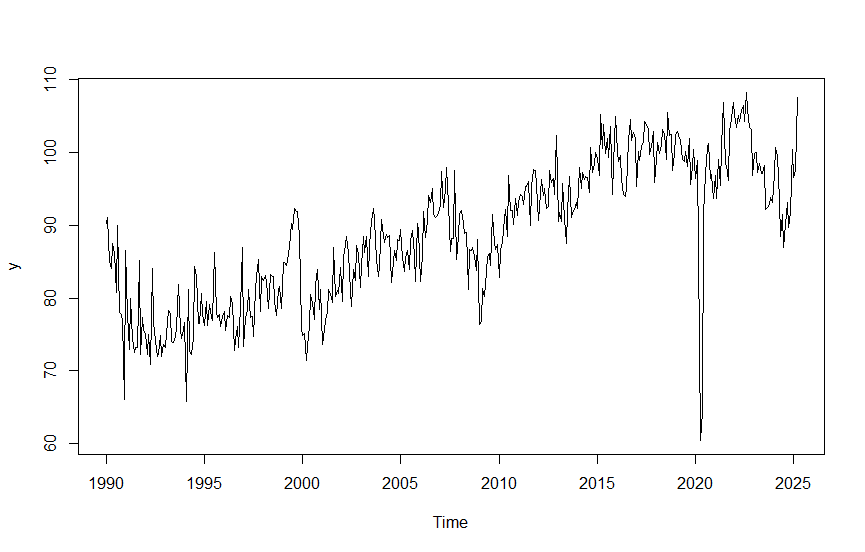
\includegraphics[width=\linewidth]{plot series.png}
                \caption{Initial series}
                \label{fig:plot_series}
            \end{subfigure}
            \hfill
            \begin{subfigure}[b]{0.49\linewidth}
                \centering
                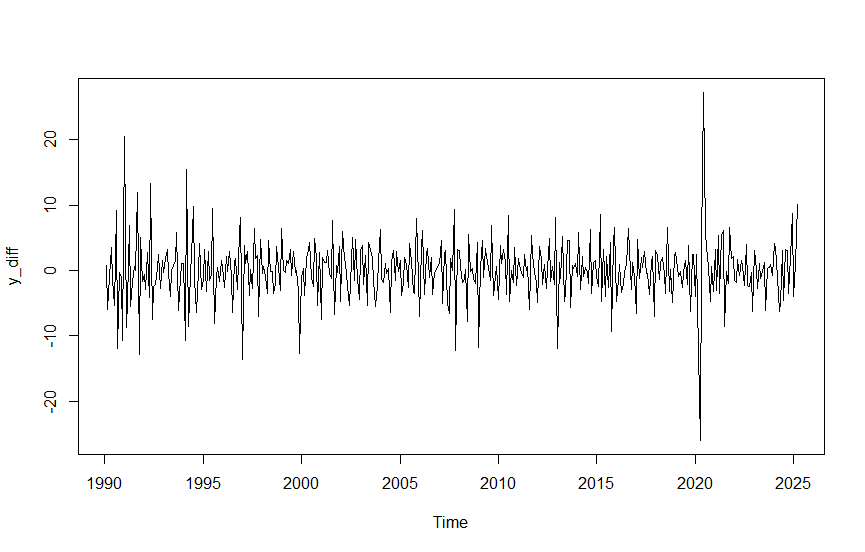
\includegraphics[width=\linewidth]{plot y_diff.png}
                \caption{First-order differenced series}
                \label{fig:plot_series_diff}
            \end{subfigure}
            \caption{Plots of the series $(Y_t)$ and $(\nabla Y_t)$}
            \label{fig:plots_two_series}
        \end{figure}

        \item The plots of the series $(Y_t)$ and $(\nabla Y_t)$ can be found on Figure \ref{fig:plots_two_series}.
    \end{enumerate}

    \section{ARMA models}

    \begin{enumerate}
        \item We seek to fit an $\ARMA(p, q)$ model on the differenced series. The autocorrelograms for the autocorrelation function (ACF) and the partial autocorrelation function (PACF) of the differenced series can be found on Figure \ref{fig:autocorrelograms}.
        %
        \begin{figure}[h]
            \centering
            \begin{subfigure}[b]{0.49\linewidth}
                \centering
                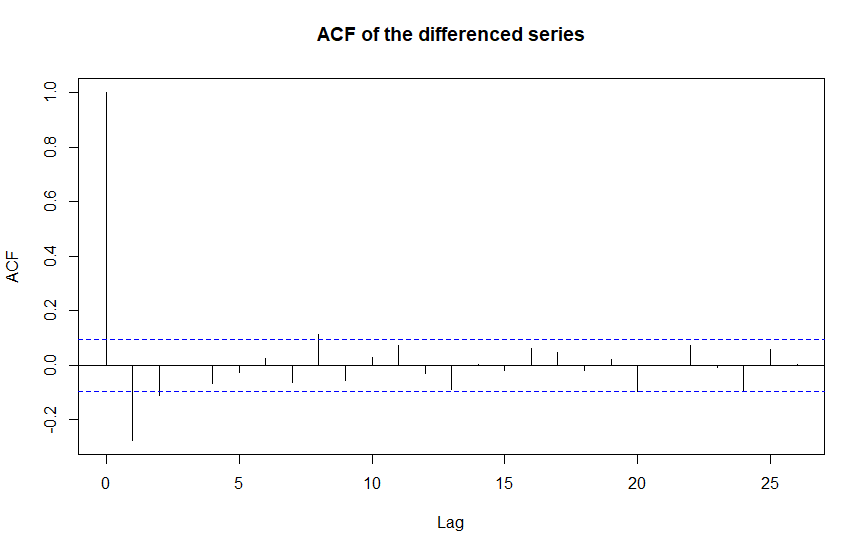
\includegraphics[width=\linewidth]{ACF ydiff.png}
                \caption{ACF of $(\nabla Y_t)$}
                \label{fig:acf_ydiff}
            \end{subfigure}
            \hfill
            \begin{subfigure}[b]{0.49\linewidth}
                \centering
                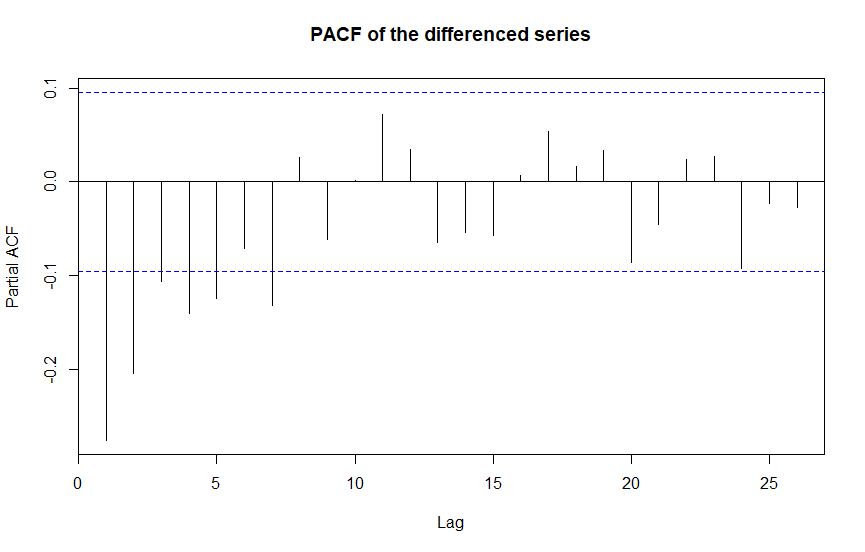
\includegraphics[width=\linewidth]{PACF ydiff.png}
                \caption{PACF of $(\nabla Y_t)$}
                \label{fig:pacf_ydiff}
            \end{subfigure}
            \caption{Autocorrelograms of the differenced series}
            \label{fig:autocorrelograms}
        \end{figure}

        Figure \ref{fig:acf_ydiff} shows that the autocorrelations become non-significant beyond lag 13, while Figure \ref{fig:pacf_ydiff} show that the partial autocorrelations become non-significant beyond lag 7. Therefore, we seek for the best $\ARMA(p, q)$ for $p = 0, 1, \dots, 7$ and $q = 0, 1, \dots, 13$. To compare those models we find $(p_{\AIC}, q_{\AIC})$ minimizing $\AIC(p, q)$ and $(p_{\BIC}, q_{\BIC})$ minimizing $\BIC(p, q)$. The results of those two minimization programs, which can be found in Table \ref{tab:aic_bic_results}, suggest that the two best candidates are $\ARMA(4, 4)$ and $\ARMA(1, 1)$. We note that, in both models, there is only one coefficient that is not statistically significant (see Table \ref{tab:arma44_coeffs} and Table \ref{tab:arma11_coeffs}). Because we foster simplest models to prevent overfitting, we choose to fit the $\ARMA(1, 1)$ model on the series $(\nabla Y_t)$ in the following.
        %
        \begin{table}[ht]
            \centering
            \begin{tabular}{l|ccc}
                \textbf{Criterion} & \textbf{Best Model} & $\AIC$ & $\BIC$ \\
                \hline
                $\AIC$  & $\ARMA(4, 4)$ & 2417.044 & 2457.494 \\
                $\BIC$  & $\ARMA(1, 1)$ & 2423.842 & 2440.022 
            \end{tabular}
            \caption{Minimization of $\AIC(p, q)$ and $\BIC(p, q)$}
            \label{tab:aic_bic_results}
        \end{table}
        %
        \begin{table}[ht]
            \centering
            \begin{tabular}{l|cccc}
                \textbf{Term} & \textbf{Estimate} & \textbf{Std. Error} & \textbf{z value} & \textbf{Pr($>|z|$)} \\
                \hline
                \rowcolor{red!15} ar1          & 0.1607  & 0.1083 & 1.4828   & 0.1381 \\
                ar2                            & 0.1814  & 0.0452 & 4.0146   & $5.95 \cdot 10^{-5}$ \\
                ar3                            & 0.8716  & 0.0228 & 38.2850  & $< 2.2 \cdot 10^{-16}$ \\
                ar4                            & -0.3651 & 0.0874 & -4.1758  & $2.97 \cdot 10^{-5}$ \\
                ma1                            & -0.6020 & 0.0913 & -6.5929  & $4.31 \cdot 10^{-11}$ \\
                ma2                            & -0.2575 & 0.0213 & -12.0644 & $< 2.2 \cdot 10^{-16}$ \\
                ma3                            & -0.8897 & 0.0259 & -34.2922 & $< 2.2 \cdot 10^{-16}$ \\
                ma4                            & 0.7492  & 0.0910 & 8.2327   & $< 2.2 \cdot 10^{-16}$ \\
                intercept                      & 0.0601  & 0.0083 & 7.2191   & $5.23 \cdot 10^{-13}$ \\
            \end{tabular}
            \caption{Coefficient estimates for $\ARMA(4, 4)$}
            \label{tab:arma44_coeffs}
        \end{table}
        %
        \begin{table}[ht]
            \centering
            \begin{tabular}{l|cccc}
                \textbf{Term} & \textbf{Estimate} & \textbf{Std. Error} & \textbf{z value} & \textbf{Pr($>|z|$)} \\
                \hline
                ar1                          & 0.4253  & 0.0815 & 5.2187   & $1.80 \cdot 10^{-7}$ \\
                ma1                          & -0.8458 & 0.0543 & -15.5889 & $< 2.2 \cdot 10^{-16}$ \\
                \rowcolor{red!15} intercept  & 0.0310  & 0.0559 & 0.5539   & 0.5796 \\
            \end{tabular}
            \caption{Coefficient estimates for $\ARMA(1, 1)$}
            \label{tab:arma11_coeffs}
        \end{table}

        To check the validity of the model we want to test whether the residual $(\varepsilon_t)$ is a white noise or not. Plotting the residuals (see Figure \ref{fig:plot_residuals}) show that it seems that it is a white noise, i.e. a zero-mean, time-independant-variance and uncorrelated sequence. To test that the residuals are uncorrelated, we use the Ljung-box test (see Table \ref{tab:ljung_box}) which accepts the null hypothesis of non-autocorrelation of the residuals at the $5 \%$ level.
        %
        \begin{figure}[h]
            \centering
            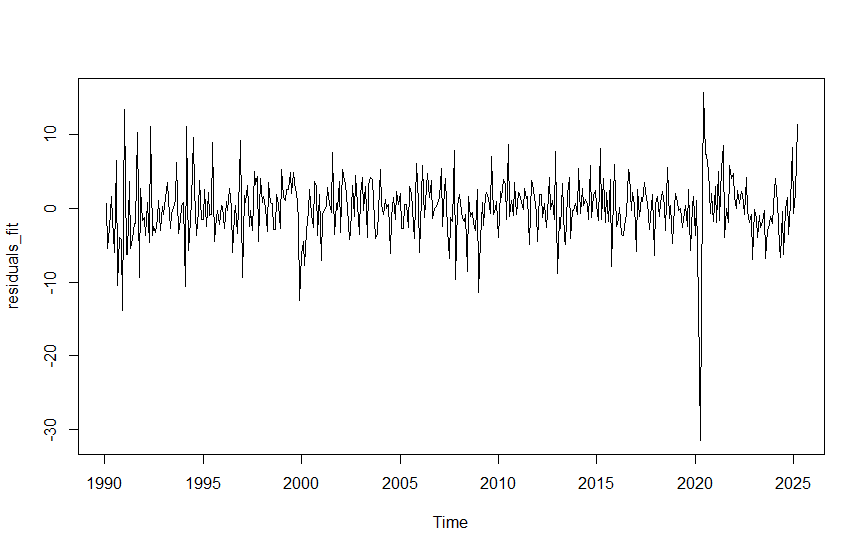
\includegraphics[width=0.5\linewidth]{plot residuals.png}
            \caption{Plot of residuals}
            \label{fig:plot_residuals}
        \end{figure}
        %
        \begin{table}[ht]
            \centering
            \begin{tabular}{l|cc}
                \textbf{df} & \(\chi^2\) & \textbf{p-value} \\
                \hline
                22 & 31.287 & 0.0904 \\
            \end{tabular}
            \caption{Ljung-Box test for lag 24 on residuals}
            \label{tab:ljung_box}
        \end{table}

        To conclude, we have picked the $\ARMA(1, 1)$ model for the series $(\nabla Y_t)$. It is valid because we have tested both the stationarity of $(\nabla Y_t)$ and the fact that the residual is a white noise.

        \item We have $(\nabla Y_t) \sim \ARMA(1, 1)$, thus $(Y_t) \sim \ARIMA(1, 1, 1)$ with the coefficient estimated in Table \ref{tab:arma11_coeffs}:
        %
        \[\nabla Y_t = 0.0310 + 0.4253 \nabla Y_{t - 1} - 0.8458 \varepsilon_{t - 1} + \varepsilon_t, \qquad (\varepsilon_t) \sim \WN(0, \sigma^2)\]
    \end{enumerate}

    \section{Prediction}

    \begin{enumerate}
        \item 
    \end{enumerate}
\end{document}